%!TEX TS-program = xelatex
\documentclass[]{friggeri-cv}
\usepackage{afterpage}
\usepackage{hyperref}
\usepackage{color}
\usepackage{xcolor}
\hypersetup{
    pdftitle={},
    pdfauthor={},
    pdfsubject={},
    pdfkeywords={},
    colorlinks=false,       % no lik border color
   allbordercolors=white    % white border color for all
}
\addbibresource{bibliography.bib}
\RequirePackage{xcolor}
\definecolor{pblue}{HTML}{0395DE}

\begin{document}
\header{Trupti}{Kini}
      {Masters In Computer Science(FOSS)}
      
% Fake text to add separator      
\fcolorbox{white}{gray}{\parbox{\dimexpr\textwidth-2\fboxsep-2\fboxrule}{%
.....
}}

% In the aside, each new line forces a line break
\begin{aside}
  \section{Address}
    B-22, First Floor, Sanman CHS, Near Sahakar Bazaar, Kharegaon, Kalwa, Thane District, 400605, Maharashtra, India

    ~
  \section{Tel}
    (+91) 9819276881
    (022) 25376435


        ~
  \section{Mail}
    \href{kinitrupti@gmail.com}{\textbf{kinitrupti@}\\gmail.com}
   
    ~
  \section{Web \& Git}
    \href{http://fossevangelist.blogspot.in/}{fossevangelist.blogspot.in/}
    \href{https://github.com/kinitrupti}{github.com/kinitrupti}
 
    ~
  \section{Programming}
    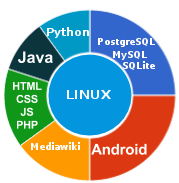
\includegraphics[scale=0.62]{img/programming.png}
    ~
  \section{OS Preference}
    \textbf{GNU/Linux}
\includegraphics[scale=0.40]{img/5stars.png}
    \textbf{Unix}
\includegraphics[scale=0.40]{img/4stars.png}
    \textbf{MacOS}
\includegraphics[scale=0.40]{img/2stars.png}
    \textbf{Windows}
\includegraphics[scale=0.40]{img/1stars.png}
    ~
  \section{Personal Skills}
    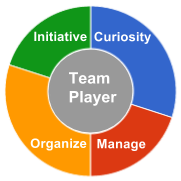
\includegraphics[scale=0.62]{img/personal.png}
    ~
\end{aside}

\section{Experience}
\begin{entrylist}
  \entry
    {2014 - Now}
    {Research Assistant and In-charge of Python Textbook Companion, FOSSEE}
    {IIT, Bombay}
    {The Textbook Companion activity aims to create a repository of reference material for Python by coding solved examples of standard engineering textbooks using Python\\
    http://python.fossee.in/about/}
    
  \entry
    {05/13 - 08/14}
    {Junior Programmer}
    {IIT, Bombay}
    {Spoken Tutorial: Created Spoken tutorials on Aakash Business Tool(ABT)\\
http://www.spoken-tutorial.org/ \\ Currently doing research and creating tutorials
on BioPython \\
Aakash Tablet: Accounting Android Application named Aakash Business Tool\\
http://aakashlabs.org/ac/project/3/\\}
    \entry
    {4/12 - 04/13}
    {Junior Programmer}
    {IIT, Bombay}
    {GNUKhata: A FOSS Accounting Web Application in Python. Contributed a
patch code for auto-updation of database. Worked on front-end using Mako and
Pylons framework\\
http://www.cometmedia.org/gnukhata
\\}
   \end{entrylist}
   
   \section{Other Languages}
\begin{entrylist}
  \entry
    {}
    {Drupal}
    {}
    {\emph{}}
     \entry
    {}
    {LaTeX}
    {}
    {\emph{}}
     \entry
    {}
    {OpenOffice}
    {}
    {\emph{}}
\end{entrylist}

   \section{Projects}
\begin{entrylist}
  \entry
    {Current}
    {MSc(CS) FOSS, Anna University portal on Mobile Platform}
    {}
    {\emph{}}
  
    
\end{entrylist}


\begin{entrylist}
  \entry
    {2014}
    {Reverse Engineering in NetBeans and performed all TestCases using JUnit, TestNG \& JMeter}
    {}
    {\emph{}}  
    
\end{entrylist}
\begin{entrylist}
  \entry
    {2013}
    {Coin toss game in Nodejs}
    {}
    {\emph{}}
  
    
\end{entrylist}



\begin{entrylist}
  \entry
    {2013}
    {Android application to get STD codes of Tamil Nadu cities}
    {}
    {\emph{}}
  
    
\end{entrylist}
\newpage
\section{Education}
\begin{entrylist}
  \entry
    {2012 - Current}
    {Master's Degree in Computer Science}
    {Anna University, Chennai}
    {Free and Open Source Software\\
    Main subjects: Software Development and Applications\\
    \emph{}\\
    \emph{}\\}
  \entry
    {2009 - 2012}
    {Bachelor's in Computer Application}
    {SNDT University, Mumbai}
    {Main subjects: Software Development\\
    \emph{}\\
    \emph{}\\}
 
\end{entrylist}



\section{Workshops}
\begin{entrylist}
  \entry
    {2012}
    {Deployment and Workshop of Project GNUKhata at AMTRON}
    {}
    {\emph{Assam}}
    \end{entrylist}
    \begin{entrylist}
     \entry
      {2012}
    {Conducted workshop on PHP, Linux, Ajax at Sanjay Ghodawat Institute}
    {}
    {\emph{Kolhapur}}
\end{entrylist}
 \begin{entrylist}
     \entry
      {2012}
    {Conducted workshop on PHP, Linux, Ajax at Rajendra Mane College Of Engineering}
    {}
    {\emph{Ratnagiri}}
\end{entrylist}
\begin{entrylist}
     \entry
      {2012}
    {Conducted workshop on PHP, Linux, Ajax at Sipna College of Engineering}
    {}
    {\emph{Amravati}}
\end{entrylist}
\begin{entrylist}
     \entry
      {2012}
    {Conducted workshop on Linux and Orca Screen Reader at Blind School}
    {}
    {\emph{Anandwan}}
\end{entrylist}

\begin{aside}
~
~
~
  \section{Places Visited}
    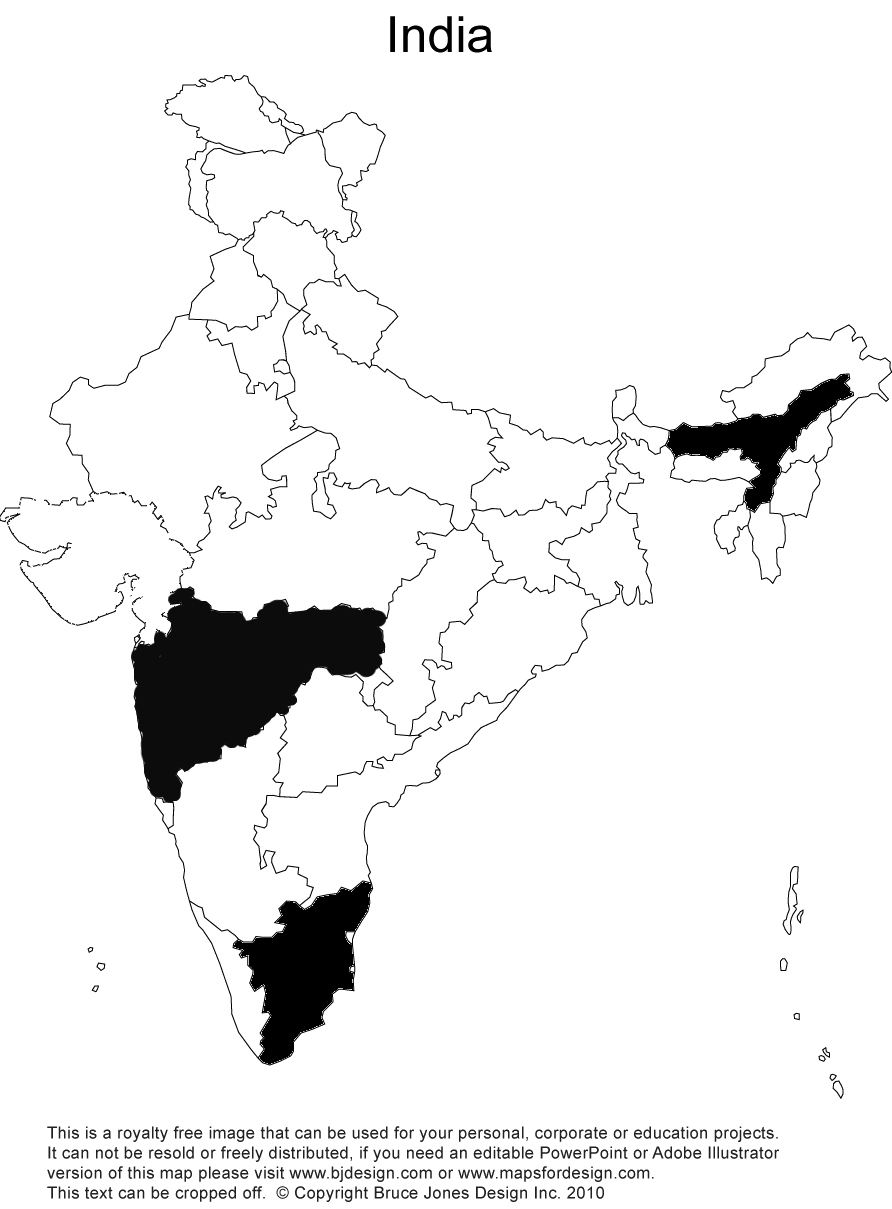
\includegraphics[scale=0.25]{img/india.jpg}
    ~
  \section{Languages}
    \textbf{English}
\includegraphics[scale=0.40]{img/5stars.png}
    \textbf{Konkani}
\includegraphics[scale=0.40]{img/5stars.png}
    \textbf{Marathi}
\includegraphics[scale=0.40]{img/5stars.png}
    \textbf{Hindi}
\includegraphics[scale=0.40]{img/4stars.png}
    \textbf{German}
\includegraphics[scale=0.40]{img/1stars.png}
\end{aside}



\section{Awards}
\begin{entrylist}
  \entry
    {2009}
    {Achieved top 10 percent rank in National Standard Examination in Biology and
Physics Olympiad}
    {}
    {\emph{}}
    \end{entrylist}
    \begin{entrylist}
     \entry
      {2012}
    {Awarded as a Most Talented Player in Sr. Level Chess Tournament Of SNDT
University}
    {}
    {\emph{}}
\end{entrylist}
 \begin{entrylist}
     \entry
      {2012}
    {Was awarded Student of the year award for my overall academic performances by
SNDT University}
    {}
    {\emph{}}
\end{entrylist}
\begin{entrylist}
     \entry
      {2012}
    {Best Anchor Award at Intercollegiate fest at BMN College, Matunga}
    {}
    {\emph{}}
\end{entrylist}
\newpage
\section{Conferences \& Publications}
\begin{entrylist}
     \entry
      {2012}
    {Attended a UGC sponsored two day state level seminar cum workshop on e-crime
and e-security by The Eagle Eye Security}
    {}
    {\emph{}}
\end{entrylist}
\begin{entrylist}
     \entry
      {2013}
    {Attended PyCon at Bangalore}
    {}
    {\emph{}}
\end{entrylist}
\begin{entrylist}
     \entry
      {2013}
    {Attended CryptoParty at VJTI, Mumbai}
    {}
    {\emph{}}
\end{entrylist}
\begin{entrylist}
     \entry
      {2013}
    {Published an article on my journey with open source technology on Red Hat website}
    {}
    {\href{http://opensource.com/life/13/4/open-source-beginnings}{opensource.com/life/13/4/open-source-beginnings}}
\end{entrylist}

\section{Interests}
\\
\begin{entrylist}
  \entry
    {.}
    {Rubiks Cube}
    {}
    {\\}
  \entry
    {}
    {Blogging}
    {}
    {\\}
    \entry
    {}
    {Trekking}
    {}
    {\\}
    \entry
    {}
    {Chess}
    {}
    {\\}
    \entry
    {}
    {Teaching}
    {}
    {\\}
    \entry
    {}
    {Skating}
    {}
    {\\}
   \end{entrylist}

\section{Extra Curricular Activities}
\\
\begin{entrylist}
  \entry
    {2009}
    {Yoga Trainer for basic Yoga Pranayams and Exercises at Ambika Yoga Kutir}
    {Matunga}
    {\\}
   \end{entrylist}
%%% This piece of code has been commented by Karol Kozioł due to biblatex errors. 
% 
%\printbibsection{article}{article in peer-reviewed journal}
%\begin{refsection}
%  \nocite{*}
%  \printbibliography[sorting=chronological, type=inproceedings, title={international peer-reviewed conferences/proceedings}, notkeyword={france}, heading=subbibliography]
%\end{refsection}
%\begin{refsection}
%  \nocite{*}
%  \printbibliography[sorting=chronological, type=inproceedings, title={local peer-reviewed conferences/proceedings}, keyword={france}, heading=subbibliography]
%\end{refsection}
%\printbibsection{misc}{other publications}
%\printbibsection{report}{research reports}

\end{document}
